\documentclass{article} % use option titlepage to get the title on a page of its own.
\usepackage{polski}
\usepackage[utf8]{inputenc}
\usepackage{graphicx}
\usepackage[a4paper, total={7in, 10in}]{geometry}
\usepackage{listings}
\graphicspath{ {./images/} }
\title{Wskaźnik Giełdowy MACD - frank szwajcarski}
\date{23.03.2018}
\author{Mateusz Buchajewicz}
\begin{document}
\maketitle
\section{Wprowadzenie}
Celem projektu było zaimplementowanie wskaźnika giełdowego MACD, wykorzystując dowolny język programowania.
Wskaźnik był sprawdzany na kursie franka szwajcarskiego w okresie od 01.04.2015 do 19.03.2019. 
Dane zaczerpnięto z serwisu money.pl. \\

\begin{figure}[h]
    \centering
    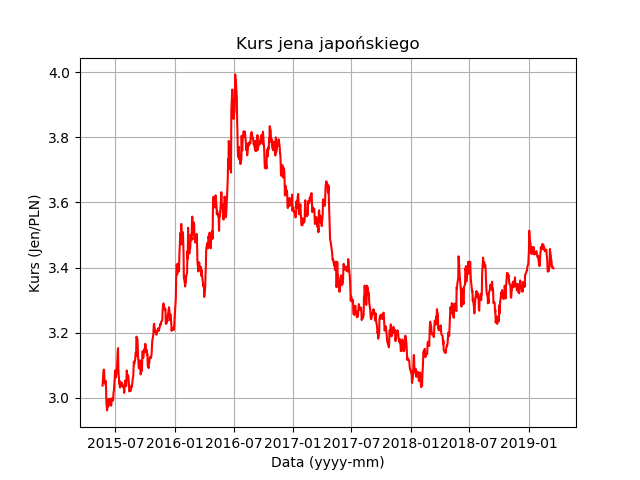
\includegraphics[scale=0.7]{wykres_kursu}
    \caption{Wykres kursu franka szwajcarskiego w okresie od 01.04.2015 do 19.03.2018.}
\end{figure} 

Ze względu na niemożliwość obliczenia składowych wskaźnika MACD dla okresu 01.04.2015 - 10.05.2015
(ze względu na brak danych z dni poprzedzających ten okres), na późniejszych wykresach jest on pomijany. \\

Do implementacji wskaźnika wykorzystano język Python. Wykresy zostały narysowane z wykorzystaniem pakietu matplotlib.




\newpage

\section{Wskaźnik MACD}
\subsection{Podstawa teoretyczna}
Wskaźnik MACD składa się z dwóch wykresów: MACD oraz linii sygnałowej SIGNAL. 
Oba opierają się na wykładniczej średniej kroczącej, określonej wzorem: \\
\begin{equation}
    EMA_{N} = \frac{p_{0} + (1-\alpha)p_{1} + \dots + (1-\alpha)^N p_{N}}{(1-\alpha) + \dots + (1-\alpha)^N}
\end{equation}
gdzie: \\ \newline
$ \alpha = \frac{2}{N - 1} $ \\
$ N $ - liczba okresów \\
$ p_{i} $ - wartość danej sprzed $ i $ dni \\


Składowa MACD jest różnicą $ EMA_{12} - EMA_{26} $ obliczoną w oparciu o dane (w tym wypadku kurs franka szwajcarskiego). 
Linia sygnałowa SINGAL jest obliczana jako $ EMA_{9} $ ze składowej MACD.

\subsection{Wykres składowych wskaźnika MACD}

\begin{figure}[h]
    \centering
    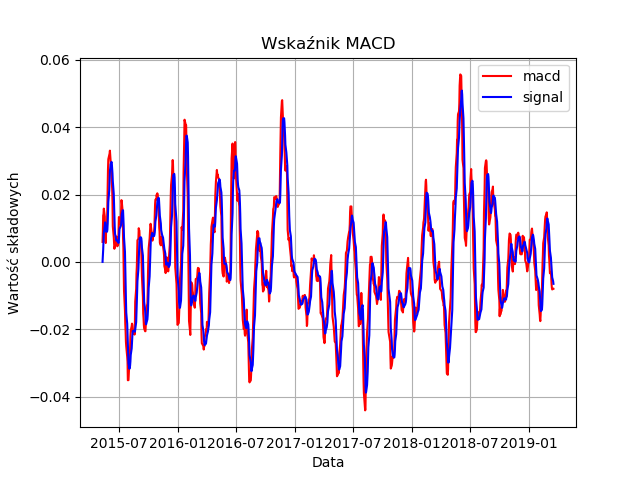
\includegraphics[scale=0.7]{images/wykres_macd.png}
    \caption{Wykres składowych wskaźnika MACD. Dane z okresu od 11.05.2015 do 19.03.2019}
\end{figure}

\newpage

\section{Analiza techniczna}


\newpage
\section{Podsumowanie}

\end{document}